\documentclass[11pt]{article}

\usepackage[margin=1in]{geometry}
\usepackage{amsmath,amssymb,amsthm}
\usepackage{booktabs}
\usepackage{enumitem}
\usepackage{graphicx}
\usepackage{hyperref}
\usepackage{placeins}
\usepackage{xcolor}

\hypersetup{
  colorlinks=true,
  linkcolor=blue,
  citecolor=blue,
  urlcolor=blue
}

\newtheorem{definition}{Definition}
\newtheorem{remark}{Remark}

\newcommand{\R}{\mathbb{R}}
\newcommand{\Cov}{\operatorname{Cov}}
\newcommand{\spanop}{\operatorname{span}}

\title{A KRR Mechanism in In-Context Transformers}
\author{Fernando Ruiz Mazo}
\date{May 1, 2026}

\begin{document}

\maketitle

\section{The Question}

A transformer can match kernel ridge regression (KRR) predictions on sampled labels without
implementing the KRR rule. Pointwise agreement tests one vector \(y\). A different computation can
agree at that vector and disagree on nearby counterfactual labels.

We therefore freeze the input geometry \(G=(X_{\mathrm{ctx}},X_{\mathrm{tgt}})\) and study the
label-response map. With \(G\) fixed, KRR is a linear operator \(T\) from context labels to target
predictions. The first question is behavioral:
\[
\text{does the transformer's local response }D_\varepsilon F(y)[u]\text{ match }Tu?
\]
The answer is only interpreted on task-distributed label directions, not on arbitrary Euclidean
perturbations.

The mechanistic question is sharper. If the transformer has a local KRR response, is that response
supported by a compact context-side residual-stream subspace? For an activation-derived basis \(Q\),
the KRR-constrained reduced operator is \(T_Q=K_tQQ^\top\). We ask whether \(T_Q\) is
prediction-equivalent to exact KRR at a predeclared posterior-risk tolerance, when such a subspace
becomes available across layers, and whether the corresponding label projection
\[
y_Q=AQQ^\top y
\]
is enough for the model to preserve the KRR-level prediction.

The claim is deliberately local. In the successful regimes, the transformer locally realizes the
task-distributed KRR label-response operator, and this behavior is explained by low-dimensional
activation subspaces whose required dimension is computed from the finite KRR task before looking at
activations. The experiments do not claim global equality with KRR or an SGD theorem for learning
the mechanism.

\section{Fixed Geometry Makes Ridge Regression an Operator}

Fix one in-context episode with context and target inputs
\[
X_{\mathrm{ctx}}\in\R^{n_{\mathrm{ctx}}\times d_x},
\qquad
X_{\mathrm{tgt}}\in\R^{n_{\mathrm{tgt}}\times d_x}.
\]
The fixed geometry is
\[
G=(X_{\mathrm{ctx}},X_{\mathrm{tgt}}).
\]
During the operator tests, \(G\) is held fixed. The context inputs do not move, the target inputs do
not move, and the only varying object is the context-label vector
\[
y=(y_1,\ldots,y_{n_{\mathrm{ctx}}})\in\R^{n_{\mathrm{ctx}}}.
\]
Define
\[
K=X_{\mathrm{ctx}}X_{\mathrm{ctx}}^\top,\qquad
K_t=X_{\mathrm{tgt}}X_{\mathrm{ctx}}^\top,\qquad
A=K+\sigma^2 I.
\]
For linear-kernel ridge regression, the dual coefficients and target predictions are
\[
\alpha^\star=A^{-1}y,\qquad
y^\star=K_t\alpha^\star=K_tA^{-1}y.
\]
Thus, once \(G\) is fixed, ridge regression is a linear map from context labels to target
predictions:
\[
T_G:=K_tA^{-1},
\qquad
T_G:\R^{n_{\mathrm{ctx}}}\to\R^{n_{\mathrm{tgt}}}.
\]

The transformer defines a map on the same spaces:
\[
F_\theta^G:\R^{n_{\mathrm{ctx}}}\to\R^{n_{\mathrm{tgt}}},
\qquad
F_\theta^G(y)=\widehat y_\theta.
\]
When the geometry is clear, write \(T\) and \(F\). The central comparison is not merely
\(F(y)\approx Ty\) for one \(y\). It is whether the local response of \(F\) to label perturbations
matches the operator \(T\).

\section{Context-Label Directions, Local Operators, and Additivity}

A context-label direction is a vector
\[
u\in\R^{n_{\mathrm{ctx}}}.
\]
It assigns one scalar to each context example. Perturbing in direction \(u\) means changing labels as
\[
y+\varepsilon u
=
(y_1+\varepsilon u_1,\ldots,y_{n_{\mathrm{ctx}}}+\varepsilon u_{n_{\mathrm{ctx}}}).
\]
This is a direction over context positions. It is not a direction in input-feature space and not a
direction in target space. If there are 47 context examples, these directions live in \(\R^{47}\).

Pointwise agreement checks only the value of two maps at one label vector:
\[
F(y)\approx Ty.
\]
Since fixed-geometry ridge regression is linear, its Jacobian is the operator itself:
\[
J_T(y)=T\quad\text{for every }y.
\]
The transformer map \(F\) can be nonlinear in the labels. The weakest local version of ``the same
label-to-prediction rule'' is therefore equality of first-order responses:
\[
J_F(y)u\approx Tu.
\]
Equivalently, for small label perturbations,
\[
F(y+\delta)\approx F(y)+T\delta.
\]
The experiments estimate the Jacobian action with the central finite difference
\[
D_\varepsilon F(y)[u]
:=
\frac{F(y+\varepsilon u)-F(y-\varepsilon u)}{2\varepsilon}.
\]
The symmetric form is used because it cancels the leading first-order bias of a one-sided
difference: for a smooth map, the error is \(O(\varepsilon^2)\) rather than \(O(\varepsilon)\). It also
treats positive and negative label perturbations in the same direction symmetrically, which is
important when the goal is to estimate the local tangent response rather than a one-sided effect.
The behavioral operator test asks whether
\[
D_\varepsilon F(y)[u]\approx Tu
\]
on held-out label directions.

This is still a local statement. Matching the value and first derivative at one point does not imply
global equality. For example, \(f(x)=x+x^2\) and \(g(x)=x\) have the same value and derivative at
\(x=0\), but differ away from zero. Thus derivative matching supports tangent-level agreement,
not \(F(y')=Ty'\) for all possible labels.

The probe distribution specifies which counterfactual label directions are tested. The main probes
are task-label probes:
\[
u\sim\mathcal{N}(0,A).
\]
This is the natural law because, under the matched linear task
\[
y=X_{\mathrm{ctx}}\beta+\eta,\qquad
\beta\sim\mathcal{N}(0,I),\qquad
\eta\sim\mathcal{N}(0,\sigma^2I),
\]
conditioning on the fixed geometry leaves only \(\beta\) and \(\eta\) random, so
\[
y\mid G\sim\mathcal{N}(0,X_{\mathrm{ctx}}X_{\mathrm{ctx}}^\top+\sigma^2I)
=\mathcal{N}(0,A).
\]
Equivalently, the conditional label covariance is
\[
\Cov(y\mid G)=A.
\]
Thus \(u\sim\mathcal{N}(0,A)\) samples counterfactual label perturbations with the same covariance
geometry as labels generated by the task, after the input geometry has been fixed. In this precise
sense, task probes are the directions the task distribution itself emphasizes. In whitened coordinates,
they are \(u=A^{1/2}z\), \(z\sim\mathcal{N}(0,I)\). The experiments also use isotropic probes
\[
u\sim\mathcal{N}(0,I),
\]
which test arbitrary context-label directions equally. The distinction is central: the claim is
task-local because the transformer is close to ridge on task-label probes but not on arbitrary
isotropic probes. Build probes are used to construct subspaces or fitted controls; held-out probes
are used for reported errors.

For a held-out probe set \(U=\{u_1,\ldots,u_m\}\) and a fixed linear operator
\(S:\R^{n_{\mathrm{ctx}}}\to\R^{n_{\mathrm{tgt}}}\), define
\[
E_\varepsilon(F,S;U)
:=
\left(
\frac{
\sum_{j=1}^m\|D_\varepsilon F(y)[u_j]-Su_j\|_2^2
}{
\sum_{j=1}^m\|Tu_j\|_2^2+\eta_{\mathrm{num}}
}
\right)^{1/2}.
\]
When \(S=T\), this measures whether the transformer's finite-difference response matches exact
ridge regression. The denominator normalizes by the ridge-response energy on the same probes, so
an error of \(0.01\) means a root-mean-square discrepancy of about one percent of the typical ridge
response size.

Because ridge is linear, its higher-order derivatives are zero. We do not try to estimate all
higher-order derivatives of the transformer. Instead, we check whether nonlinear interactions are
small at the tested perturbation scale. Ridge has
\[
T(u+v)=Tu+Tv.
\]
A nonlinear transformer need not satisfy
\[
D_\varepsilon F(y)[u+v]\approx D_\varepsilon F(y)[u]+D_\varepsilon F(y)[v].
\]
If this approximate additivity failed badly, then \(E_\varepsilon(F,T)\) would mix two effects:
failure to be ridge and failure to have a stable local linear response.

For paired directions \(V=\{(u_j,v_j)\}_{j=1}^m\), define the second mixed finite difference
\[
C_j =
F(y+\varepsilon u_j+\varepsilon v_j)
-F(y+\varepsilon u_j-\varepsilon v_j)
-F(y-\varepsilon u_j+\varepsilon v_j)
+F(y-\varepsilon u_j-\varepsilon v_j),
\]
and the additivity defect
\[
A_\varepsilon(F;V)
:=
\left(
\frac{
\sum_{j=1}^m\|C_j\|_2^2
}{
\sum_{j=1}^m\|T(\varepsilon u_j+\varepsilon v_j)\|_2^2+\eta_{\mathrm{num}}
}
\right)^{1/2}.
\]
For any affine function of the labels, \(C_j=0\) exactly. Because the defect is normalized by
ridge-response energy, values below one mean the non-additive interaction is smaller than the
typical ridge response on the tested paired probes; values around one mean it is ridge-scale; values
above one mean the interaction is larger than the ridge response, so a local-linear interpretation is
unreliable. This diagnostic does not identify the operator. It only says whether a local operator
comparison is meaningful at the chosen \(\varepsilon\) and probe law.

\section{Activation Subspaces and Prediction-Risk Rank}

The previous section gives behavioral certificates:
\[
F(y)\approx Ty,\qquad D_\varepsilon F(y)[u]\approx Tu.
\]
These are necessary, but they are still input-output facts. They do not say whether the transformer
represents the directions needed for ridge regression, or whether those directions are used. The
mechanistic question is: does the residual stream expose a compact set of context-position
directions sufficient for the prediction-relevant ridge computation?

This is the right internal object to look for because ridge uses context-position dual variables.
For fixed geometry,
\[
\alpha^\star(y)=A^{-1}y\in\R^{n_{\mathrm{ctx}}},
\qquad
Ty=K_t\alpha^\star(y).
\]
The dual coordinate \(\alpha_i\) is indexed by the \(i\)-th context example. The context residual
stream has the same context axis. At layer \(\ell\),
\[
H_\ell^{\mathrm{ctx}}\in\R^{n_{\mathrm{ctx}}\times D},
\]
where \(D\) is the residual width. Rows are context tokens, and the \(k\)-th column
\(H_\ell^{\mathrm{ctx}}[:,k]\) is a scalar pattern over context positions, hence a vector in
\(\R^{n_{\mathrm{ctx}}}\). Linear combinations of residual-stream columns therefore define
candidate directions in the same space as ridge dual variables.

Let
\[
Q=[q_1,\ldots,q_r]\in\R^{n_{\mathrm{ctx}}\times r}
\]
be a basis matrix for such candidate context-position directions. The subspace is the column span
\[
\spanop(Q)=\{Qc:c\in\R^r\}\subseteq\R^{n_{\mathrm{ctx}}},
\]
so \(Q\) is both a matrix representation and, by abuse of language, the subspace it spans. We use
an \(A\)-orthonormal basis,
\[
Q^\top A Q=I,
\]
because the quadratic part of the ridge dual objective is \(\frac12\alpha^\top A\alpha\). Thus the
natural size of a dual displacement is \(\alpha^\top A\alpha\), and two directions are orthogonal in
the ridge geometry when their cross-term in this quadratic energy vanishes.

Now define what it means for \(\spanop(Q)\) to be useful for ridge. This is a restriction of the
dual solution, not an ordinary restriction of the input label vector. Full ridge solves
\[
\alpha^\star(y)
=
\arg\min_{\alpha\in\R^{n_{\mathrm{ctx}}}}
\left\{
\frac12\alpha^\top A\alpha-\alpha^\top y
\right\},
\]
whose first-order condition is \(A\alpha-y=0\), hence \(\alpha^\star=A^{-1}y\). To restrict the
dual solution to \(\spanop(Q)\), write \(\alpha=Qc\). Plugging this into the same dual objective gives
\[
\frac12 c^\top Q^\top A Qc-c^\top Q^\top y.
\]
Since \(Q^\top A Q=I\), this is
\[
\frac12 c^\top c-c^\top Q^\top y.
\]
Differentiating with respect to \(c\) gives \(c-Q^\top y=0\), so
\[
c^\star=Q^\top y.
\]
Therefore the restricted dual solution is
\[
\alpha_Q(y)=QQ^\top y.
\]
Without the \(A\)-orthonormal convention, the same calculation would give
\[
\alpha_Q(y)=Q(Q^\top A Q)^{-1}Q^\top y.
\]
Predictions are still read out through the context-target kernel matrix \(K_t\), so the reduced
ridge operator induced by \(Q\) is
\[
T_Q:=K_tQQ^\top.
\]
This is the bridge from residual-stream directions to an operator-level certificate. We are not
fitting an arbitrary probe. We are asking whether the directions exposed by the residual stream are
enough so that ridge, restricted to those directions, still predicts like full ridge.

The reason this sufficiency test is prediction-relevance weighted rather than global is that not
every label direction matters equally for prediction. Conditional on the fixed geometry,
\[
y\mid G\sim\mathcal{N}(0,A).
\]
So the task naturally emphasizes perturbations
\[
u\sim\mathcal{N}(0,A),
\]
not arbitrary Euclidean directions. A direction is task-relevant when it is likely under this
covariance geometry and when ridge produces a non-negligible target response along it. This leads
to a purely ridge-theoretic benchmark: before looking inside the transformer, ask how many
directions are needed by the best possible reduced ridge response on task-distributed labels.

To turn this into a prediction-scale benchmark, we need a reference risk. The target quantity is not
the noisy context-label vector \(y\). It is the vector of latent, noise-free function values at the
target inputs. Write
\[
f_{\mathrm{tgt}}
=
\bigl(f(x^{\mathrm{tgt}}_1),\ldots,f(x^{\mathrm{tgt}}_{n_{\mathrm{tgt}}})\bigr)
\in\R^{n_{\mathrm{tgt}}},
\]
and let \(K_{tt}\) be the target-target kernel matrix. In the linear case,
\(K_{tt}=X_{\mathrm{tgt}}X_{\mathrm{tgt}}^\top\). Under the matched GP/KRR model,
\[
\begin{bmatrix}
y\\
f_{\mathrm{tgt}}
\end{bmatrix}
\Bigm|G
\sim
\mathcal{N}\!\left(
0,
\begin{bmatrix}
A & K_t^\top\\
K_t & K_{tt}
\end{bmatrix}
\right),
\]
because \(y=f_{\mathrm{ctx}}+\eta\) includes label noise while \(f_{\mathrm{tgt}}\) is the
noise-free target function. Conditioning this Gaussian gives
\[
\mathbb{E}[f_{\mathrm{tgt}}\mid y,G]=K_tA^{-1}y=Ty
\]
and
\[
\operatorname{Cov}(f_{\mathrm{tgt}}\mid y,G)
=
K_{tt}-K_tA^{-1}K_t^\top .
\]
Thus exact KRR is the posterior mean predictor of the latent target values. It still has nonzero
risk, because the noisy context labels do not determine the target function values exactly. Define
this irreducible KRR posterior prediction risk by
\[
R_{\mathrm{KRR}}(G)
:=
\mathbb{E}\|f_{\mathrm{tgt}}-Ty\|_2^2
=
\operatorname{tr}\!\left(K_{tt}-K_tA^{-1}K_t^\top\right),
\]
where the expectation is conditional on the fixed geometry \(G\).

Now compare exact KRR with any linear approximation \(S\) to \(T\). Decompose
\[
f_{\mathrm{tgt}}-Sy
=
\bigl(f_{\mathrm{tgt}}-Ty\bigr)
+
\bigl(T-S\bigr)y.
\]
The first term is the posterior residual after exact KRR, and the second term is a function of the
observed labels \(y\). Since \(Ty=\mathbb{E}[f_{\mathrm{tgt}}\mid y,G]\), the posterior residual is
orthogonal to every function of \(y\). Therefore the cross-term vanishes and
\[
\mathbb{E}\|f_{\mathrm{tgt}}-Sy\|_2^2
=
R_{\mathrm{KRR}}(G)
+
\mathbb{E}_{y\sim\mathcal{N}(0,A)}\|(T-S)y\|_2^2.
\]
The second term is the extra prediction risk caused by using \(S\) instead of exact KRR. Thus the
natural scale for deciding whether a reduced operator is good enough is not zero operator error, but
excess error relative to the irreducible risk already incurred by exact KRR. Define
\[
\rho_G(S)
:=
\frac{
\mathbb{E}_{y\sim\mathcal{N}(0,A)}\|(T-S)y\|_2^2
}{
R_{\mathrm{KRR}}(G)+\eta_{\mathrm{num}}
}.
\]
This asks how much prediction risk is added by using \(S\) instead of exact KRR.

The rank benchmark should also be defined before looking at activations. The right baseline is not
zero error: exact KRR is already uncertain about the latent target values, with posterior risk
\(R_{\mathrm{KRR}}(G)\). Therefore a reduced operator should be called sufficient when its discarded
KRR response adds only a small fraction of that unavoidable risk.

To make this intrinsic to the task distribution, put task-label perturbations in whitened
coordinates:
\[
u=A^{1/2}z,\qquad z\sim\mathcal{N}(0,I).
\]
In these coordinates exact KRR acts as
\[
Tu=K_tA^{-1}A^{1/2}z
=K_tA^{-1/2}z.
\]
Define the whitened KRR response operator
\[
C_G:=K_tA^{-1/2}.
\]
This is not a different predictor; it is \(T\) written in coordinates where the label directions
generated by the task are spherical. This is why the spectrum of \(C_G\), not the raw Euclidean
spectrum of \(T\), is the relevant one for task-local difficulty.

Let
\[
C_G=U\operatorname{diag}(s_i)V^\top,
\qquad
s_1\ge s_2\ge\cdots\ge0.
\]
The right singular vectors \(v_i\) are the task-label modes seen by KRR, and \(s_i^2\) is the target
response energy carried by mode \(i\). Since \(z\) is isotropic,
\[
\mathbb{E}\|C_Gz\|_2^2=\sum_i s_i^2.
\]
Among all rank-\(r\) linear responses in these whitened coordinates, Eckart--Young says that the best
one keeps the first \(r\) singular modes. Its unavoidable excess prediction error is exactly the
discarded tail
\[
\sum_{i>r}s_i^2.
\]
Thus the best rank-\(r\) reduced KRR predictor has total prediction risk
\[
R_{\mathrm{KRR}}(G)+\sum_{i>r}s_i^2.
\]
The tail is compared to \(R_{\mathrm{KRR}}(G)\) because the practical question is prediction
equivalence: does removing the remaining modes add little error relative to the uncertainty that KRR
cannot remove anyway?

\begin{definition}[Prediction-risk rank]
For fixed geometry \(G\) and tolerance \(\alpha>0\), define
\[
r_\alpha(G)
:=
\min\left\{
r:
\sum_{i>r}s_i^2
\le
\alpha R_{\mathrm{KRR}}(G)
\right\}.
\]
\end{definition}

In the experiments below we write \(r_T:=r_{5\%}\), i.e. \(\alpha=0.05\). Thus \(r_T\) is the smallest
rank for which the best reduced KRR response would have prediction risk at most
\[
(1.05)\,R_{\mathrm{KRR}}(G).
\]
It is not the algebraic rank of \(T\), nor the number of nonzero singular values. It is the number of
task-visible KRR modes needed to be prediction-equivalent to exact KRR at the chosen tolerance.
Modes beyond \(r_T\) may be nonzero, but their combined contribution is below the risk budget.

This is a finite-episode benchmark. It is computed from the sampled matrices \(K,K_t,K_{tt}\) before
looking at the transformer. The same definition applies to nonlinear kernels by replacing these with
the corresponding finite kernel matrices; no population spectral assumption is required.

Activation subspaces are then tested against this benchmark. Let \(Q\) be an \(A\)-orthonormal
candidate basis, \(Q^\top A Q=I\), and set
\[
C_G=K_tA^{-1/2},\qquad W=A^{1/2}Q,\qquad P_Q=WW^\top .
\]
Here \(W\) is the same context-side subspace expressed in whitened task-label coordinates. For
\(u=A^{1/2}z\),
\[
Tu=C_Gz,\qquad
T_Qu=K_tQQ^\top A^{1/2}z=C_GP_Qz.
\]
Therefore the prediction-risk excess of the reduced operator is
\[
\rho_G(T_Q)
=
\frac{\|C_G(I-P_Q)\|_F^2}{R_{\mathrm{KRR}}(G)+\eta_{\mathrm{num}}}.
\]
If \(W\) spans the top \(r\) right singular directions of \(C_G\), then
\[
\rho_G(T_Q)
=
\frac{\sum_{i>r}s_i^2}{R_{\mathrm{KRR}}(G)+\eta_{\mathrm{num}}}.
\]
This formula is the bridge from \(r_T\) to activations. If \(\dim\spanop(Q)<r_T\), the subspace
cannot reach the five-percent prediction-risk tolerance. If \(\dim\spanop(Q)\ge r_T\), success still
requires alignment: \(A^{1/2}\spanop(Q)\) must contain the leading task-label modes of \(C_G\).

\begin{remark}[Reading the numbers]
The number \(\rho_G(S)\) is an excess-risk ratio. Thus \(\rho_G(S)=0.05\) means that using \(S\)
instead of exact KRR adds five percent of the KRR posterior prediction risk. Values near zero mean
the reduced operator is prediction-equivalent to KRR at the chosen tolerance. Values near or above
one mean that the reduction adds error comparable to, or larger than, the irreducible KRR risk.
Transformer response errors \(E_\varepsilon(F,T)\) and \(E_\varepsilon(F,T_Q)\) are different
finite-difference diagnostics and are not bounded by this risk scale.
\end{remark}

The mechanism argument therefore needs three distinct checks:
\[
E_\varepsilon(F,T;U)\ \text{small},
\qquad
\rho_G(T_Q)\ \text{small},
\qquad
E_\varepsilon(F,T_Q;U)\ \text{small}.
\]
The first is behavioral. The second says the residual-stream subspace supports ridge in the
prediction-risk sense. The third says the transformer's local response follows the reduced
operator induced by that same subspace. The decomposition
\[
D_\varepsilon F(y)[u]-Tu
=
\bigl(D_\varepsilon F(y)[u]-T_Qu\bigr)
+
\bigl(T_Qu-Tu\bigr)
\]
keeps these claims separate.

It remains to describe how the residual-stream subspace is extracted. The experiments use two
final-state constructions in this section, and the next section introduces the layerwise
construction. Given any context-pattern
matrix \(M\in\R^{n_{\mathrm{ctx}}\times p}\), compute the \(A\)-weighted SVD
\[
A^{1/2}M=U\Sigma V^\top,
\]
keep the selected left singular directions, and map back:
\[
Q(M):=A^{-1/2}U_{\mathrm{kept}}.
\]
Then \(Q(M)^\top A Q(M)=I\). The ordered prefixes of this basis define a rank curve. The
prediction-risk rank tells how many ridge-relevant directions should be enough in principle; the
experiments then ask where the residual-stream prefixes first achieve small \(\rho_G(T_Q)\).

The raw final-state extractor uses the unperturbed final residual stream,
\[
M_{\mathrm{raw}}=H_L^{\mathrm{ctx}},
\qquad
Q_{\mathrm{raw}}:=Q(M_{\mathrm{raw}}).
\]
It asks an availability question: which context-position directions are linearly visible in the final
residual stream, and are enough of them present to support the prediction-relevant ridge operator?

The response-only extractor uses finite-difference changes in the final residual stream,
\[
Z_L(u)=
\frac{
H_L^{\mathrm{ctx}}(y+\varepsilon u)-H_L^{\mathrm{ctx}}(y-\varepsilon u)
}{2\varepsilon},
\qquad
M_{\mathrm{resp}}=[Z_L(u_1),\ldots,Z_L(u_m)],
\]
and sets
\[
Q_{\mathrm{resp}}:=Q(M_{\mathrm{resp}}).
\]
It asks the stricter question: among the directions that actually move when labels are perturbed,
is there a context-position subspace whose induced \(T_Q\) has small prediction-risk excess?

In both constructions \(Q\) is frozen after extraction. If the basis were re-extracted for each
held-out perturbation, it would not define one stable reduced operator. The certificate is that a
fixed subspace extracted from residual-stream activations induces a fixed \(T_Q\) that is
prediction-risk sufficient and whose action matches the transformer's held-out local response.

\section{Layerwise Availability Construction}

The final-state certificate can show that a useful subspace is present at the end of the computation,
but it does not explain how that subspace appears across layers. The revised layerwise construction
is a post-training diagnostic for this question. It asks, at each layer, whether the layer's
label-response span contains a subspace of approximately \(r_T\) dimensions whose induced reduced
KRR operator reaches the prediction-risk tolerance.

This replaces one-at-a-time direction selection as the primary emergence definition: a distributed
representation can contain the right subspace while no single arbitrary basis direction is
individually necessary. The layerwise sufficiency construction first finds a KRR-sufficient
subspace; the later label-space tests then ask whether the selected subspace carries the useful
labels.

At layer \(\ell\), define the hidden-state finite-difference response
\[
Z_\ell(u)
:=
\frac{
H_\ell^{\mathrm{ctx}}(y+\varepsilon u)-H_\ell^{\mathrm{ctx}}(y-\varepsilon u)
}{2\varepsilon}.
\]
Stacking these matrices over build probes gives
\[
M_\ell=[Z_\ell(u_1),\ldots,Z_\ell(u_m)].
\]
The columns of \(M_\ell\) are context-position patterns that are visible at layer \(\ell\) when
context labels move. An \(A\)-weighted SVD proposes an \(A\)-orthonormal candidate response span
\[
A^{1/2}M_\ell=U_\ell\Sigma_\ell V_\ell^\top,
\qquad
q_i=A^{-1/2}U_{\ell,i}.
\]
Keeping the singular directions above a numerical threshold gives a candidate span \(C_\ell\). This
span is activation-derived. The next step is deliberately KRR-targeted: given the directions that the
transformer makes available at layer \(\ell\), we ask whether that span contains a
KRR-sufficient subspace of the intrinsic task rank. This question is necessarily oracle-guided with
respect to exact KRR, because ``KRR-sufficient'' is defined by the excess-risk metric
\(\rho_G\). We therefore order directions inside \(C_\ell\) by KRR usefulness. If \(C_\ell\) is
represented by an \(A\)-orthonormal matrix, set
\[
W_\ell=A^{1/2}C_\ell,
\qquad
Z=K_tA^{-1/2}.
\]
The eigenvectors of
\[
W_\ell^\top Z^\top ZW_\ell
\]
ordered from largest to smallest define nested prefixes
\[
Q_{\ell,0}\subset Q_{\ell,1}\subset\cdots\subset C_\ell.
\]
This ordering does not claim that the transformer itself has chosen this basis. It is an availability
test: among the response directions exposed by the transformer, how good is the best KRR-aligned
prefix?
For each prefix we form
\[
T_{Q_{\ell,k}}=K_tQ_{\ell,k}Q_{\ell,k}^\top
\]
and evaluate
\[
\rho_G(T_{Q_{\ell,k}})
=
\frac{\|(T-T_{Q_{\ell,k}})A^{1/2}\|_F^2}{R_{\mathrm{KRR}}+\eta_{\mathrm{num}}}.
\]
The two ranks in the experiment have different meanings. The prediction-risk rank
\(r_T(G;0.05)\) is intrinsic to the finite KRR task: it is computed from
\(C_G=K_tA^{-1/2}\) before looking at the transformer. It is the smallest optimal rank that leaves
at most five percent of KRR posterior risk in the discarded tail. By contrast, the layerwise
rank-to-five-percent
\[
k_\ell^{5\%}
:=
\min\{k:\rho_G(T_{Q_{\ell,k}})\le0.05\}
\]
is representation-dependent: it asks how many directions from the transformer's candidate response
span \(C_\ell\) are needed to reach the same risk tolerance. If \(k_\ell^{5\%}\approx r_T\), then
the layer contains an almost optimally aligned KRR subspace. If \(k_\ell^{5\%}\gg r_T\), the span
contains relevant information but in a poorly aligned form. If no such \(k\) exists, that layer's
candidate span is not sufficient. We also report \(\rho_G(T_{Q_{\ell,r_T}})\), the excess risk of
using exactly the intrinsic task rank, and the best excess achievable inside \(C_\ell\).

\section{Experiment 1: Final-State Operator Certificate}

The experiments are organized as an evidence ladder. Experiment 1 first certifies that the
trained model has a task-local ridge-like response at the final output and that this response is
explained by a compact final-state context subspace. Experiment 2 asks where such a subspace becomes
available across layers. Experiment 3 tests on-manifold use by feeding the label projection
\(y_Q=AQQ^\top y\); Experiment 4 uses the same projection as a conditional repair test.
All checkpoint names below refer to the archived final checkpoints under \path{checkpoints/final/};
when useful, we also give the original training artifact.

We use the same metric conventions throughout the tables. \(E(F,S)\) always denotes the
finite-difference operator error between the transformer's local label response and a comparison
operator \(S\), normalized by exact-KRR response energy on the same held-out probes; subscripts such
as \(E_{\mathrm{task}}\) and \(E_{\mathrm{iso}}\) specify the probe distribution. \(\rho_G(S)\) is
the exact KRR prediction-risk excess of \(S\), normalized by the posterior KRR risk. Pointwise
prediction errors are different: they use the unperturbed label vector \(y\), for example
\(\|F(y)-Ty\|/\|Ty\|\). Thus \(E\) measures a local operator, while pointwise errors measure one
episode's actual prediction.

The first step is deliberately narrow. For each episode, the geometry \(G\) is fixed, exact KRR is
the operator \(T=K_tA^{-1}\), and the transformer is probed only by infinitesimal context-label
perturbations. Build probes are used to extract the raw and response final-state bases; all reported
errors use held-out task-label probes after the basis is frozen.

The trained model is \path{linear_baseline_dx5_L8.pt}, copied from the original
\path{checkpoints/model_L8.pt}. It is an 8-layer linear-regression ICL transformer with \(d_x=5\),
residual width \(D=128\), 4 attention heads, and no layer normalization. The evaluation uses the
linear kernel
\[
K=X_{\mathrm{ctx}}X_{\mathrm{ctx}}^\top,
\qquad
K_t=X_{\mathrm{tgt}}X_{\mathrm{ctx}}^\top,
\]
with \(n_{\mathrm{ctx}}=47\), \(n_{\mathrm{tgt}}=3\), and \(\sigma^2=0.1\). Episode geometries are
drawn from the same flat-spectrum linear family used by the baseline sampler: for each episode,
\[
c\sim\mathrm{Unif}[1,10],
\qquad
x_i\sim\mathcal{N}(0,cI_5),
\qquad
\beta\sim\mathcal{N}(0,I_5),
\]
with \(y_i=x_i^\top\beta+\epsilon_i\), \(\epsilon_i\sim\mathcal{N}(0,\sigma^2)\), on context
positions and noiseless teacher values on target positions. The reported run uses 4 episodes, 16
build probes, 32 held-out probes, and finite-difference scale \(\varepsilon=10^{-3}\).

Raw and response bases are built as ordered \(A\)-weighted SVD prefixes. Rather than imposing a
fixed rank cap, we evaluate the rank-prefix curve and select the first prefix whose reduced
operator reaches the prediction-risk tolerance,
\[
\rho_G(T_Q)\le0.05.
\]
This gives rank \(6\) for both raw and response bases in the reported run. The larger curve is still
shown, so the reader can see where the subspace becomes sufficient and whether additional
directions materially change the conclusion.

The endpoint certificate has three parts. First, the model's local response is already close to
KRR on task-label directions. Second, the activation-derived subspace induces a KRR-structured
operator \(T_Q=K_tQQ^\top\) whose prediction-risk excess is far below the five-percent tolerance.
Third, this is not merely a decodability result: a same-span least-squares readout can fit the
model response slightly better, but it is much less KRR-like.
In Table~\ref{tab:exp1-certificate}, \(k_{\rho\le5\%}\) is the first prefix rank whose
\(\rho_G(T_Q)\le0.05\). The actLR control uses the same activation coordinates \(Q^\top u\) but
learns a free least-squares readout to match the transformer's finite-difference responses; it
therefore tests decodability without imposing the KRR readout \(K_tQ\). Matched random subspaces
are random \(A\)-orthonormal subspaces with the same rank as the extracted basis.

\begin{table}[htbp]
\centering
\caption{Experiment 1 endpoint certificate, mean over 4 episodes. \(E(F,S)\) is the held-out
finite-difference operator error on task-label probes. \(\rho_G(S)\) is exact prediction-risk excess
relative to KRR.}
\label{tab:exp1-certificate}
\small
\setlength{\tabcolsep}{4pt}
\begin{tabular}{@{}p{0.30\linewidth}p{0.30\linewidth}p{0.32\linewidth}@{}}
\toprule
Check & Result & Reading\\
\midrule
Model vs. exact KRR &
\(E_{\mathrm{task}}(F,T)=0.01259\); pointwise discrepancy \(0.01045\) &
The checkpoint is locally KRR-like on task-label perturbations.\\
Raw final basis &
\(k_{\rho\le5\%}=6\), \(\rho_G(T_Q)=0.00439\), \(E_{\mathrm{task}}(F,T_Q)=0.01218\) &
The final residual stream contains a highly sufficient KRR source subspace.\\
Response final basis &
\(k_{\rho\le5\%}=6\), \(\rho_G(T_Q)=0.01651\), \(E_{\mathrm{task}}(F,T_Q)=0.01343\) &
The sufficient subspace is also visible in label-induced hidden-state motion.\\
Same-span readout control &
raw: \(E_{\mathrm{task}}(F,T_{\mathrm{actLR}})=0.00765\), \(\rho_G(T_{\mathrm{actLR}})=0.14676\) &
A free readout can fit the model, but the KRR-constrained readout is the one that remains KRR-like.\\
Matched random subspaces &
\(\rho_G(T_Q)\approx50.3\) at raw rank, \(\approx23.9\) at response rank &
Sufficiency is not explained by rank alone.\\
Isotropic label probes &
\(E_{\mathrm{iso}}(F,T)\approx0.294\) &
The certificate is task-local, not a global equality with ridge regression.\\
\bottomrule
\end{tabular}
\end{table}

Figure~\ref{fig:exp1-rank-curves} shows the rank diagnostic behind the compactness claim. The
x-axis increases the number of \(A\)-weighted SVD prefix directions used to form \(Q\). The dashed
line marks the first rank at which the task-label reduced operator satisfies
\(\rho_G(T_Q)\le0.05\), averaged over raw and response bases. The task-label curves collapse by
ranks \(5\)--\(6\): at that point the reduced operator is prediction-risk sufficient, and the
model-to-\(T_Q\) finite-difference error is already at its plateau.

\begin{figure}[htbp]
\centering
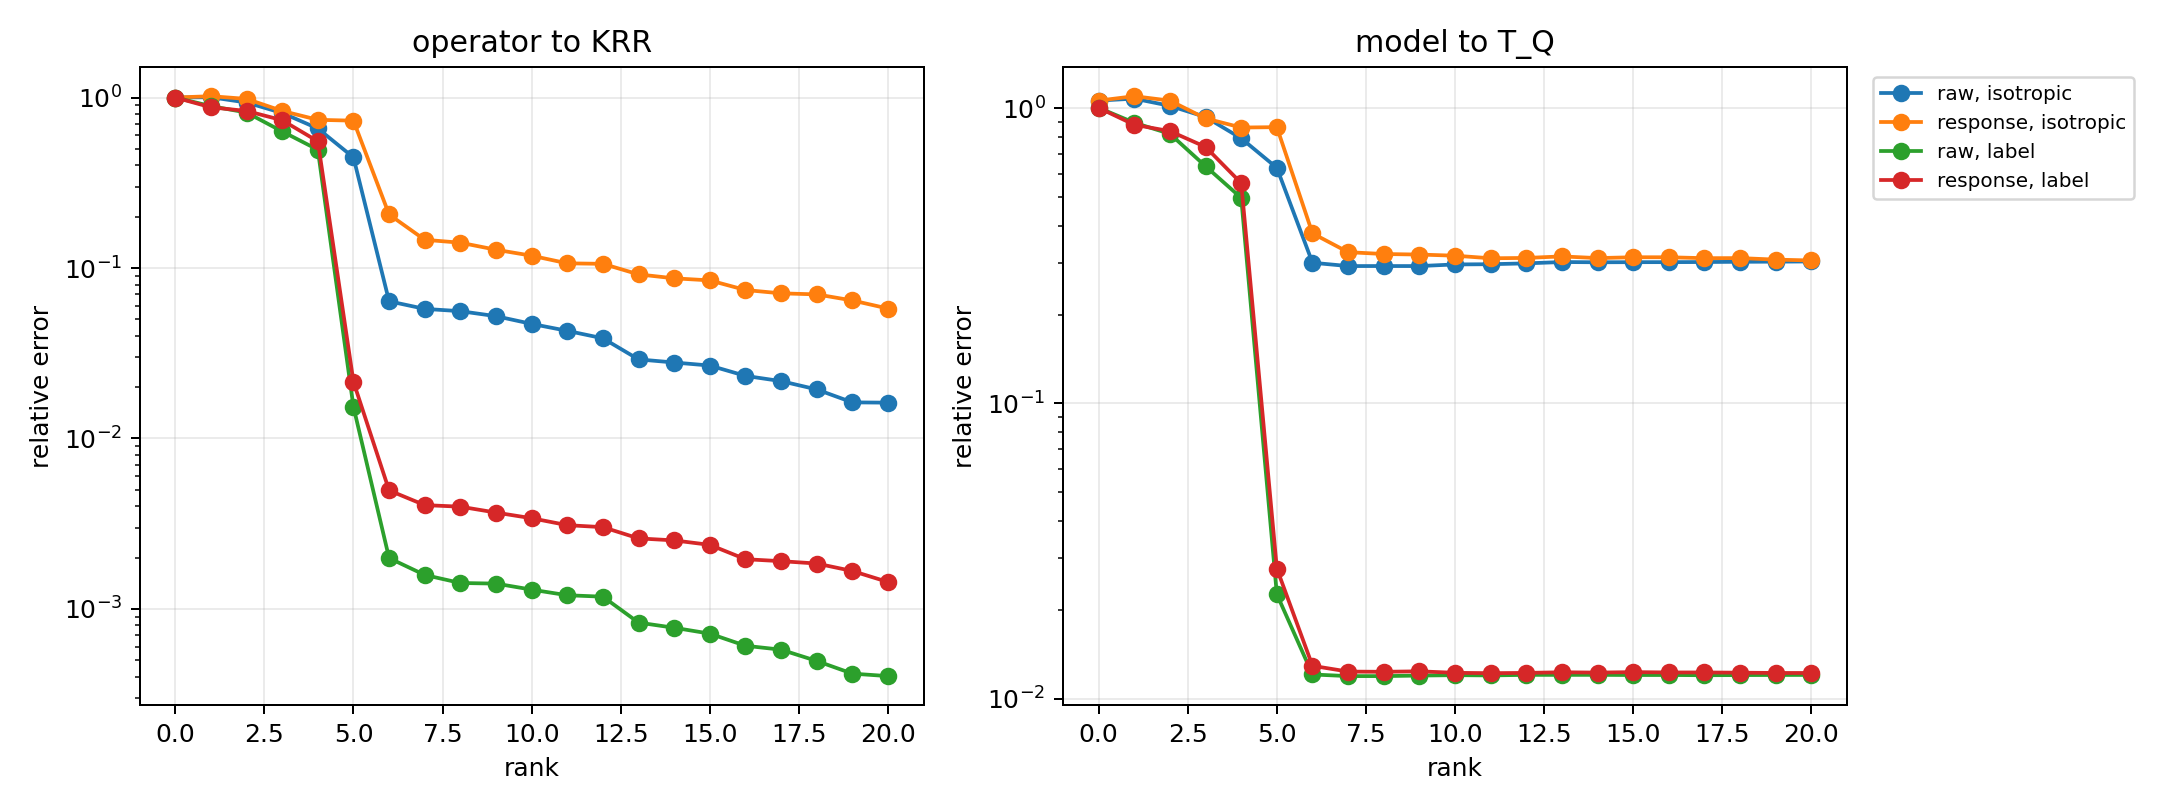
\includegraphics[width=0.92\linewidth]{../experiments/experiment_1_operator_certificate/results/rank_curves.png}
\caption{Experiment 1 rank-prefix curves. Left: prediction-risk excess \(\rho_G(T_Q)\), with the
dotted line marking the five-percent tolerance. Right: held-out task-probe response error
\(E_{\mathrm{task}}(F,T_Q)\). The dashed vertical line marks the first prediction-risk-sufficient
prefix, \(k_{\rho\le5\%}=6\); the plotted ranks are prefixes of the same \(A\)-weighted SVD basis.}
\label{fig:exp1-rank-curves}
\end{figure}

Figure~\ref{fig:exp1-actlr-control} visualizes the same-span readout control. The free
activation-low-rank readout can reduce model-response error, especially on task probes, but it pays
for that flexibility in prediction-risk excess. The KRR-constrained \(T_Q\) is therefore the
stronger certificate: the activation coordinates do not merely decode the model's response; they
support the KRR readout.

\begin{figure}[htbp]
\centering
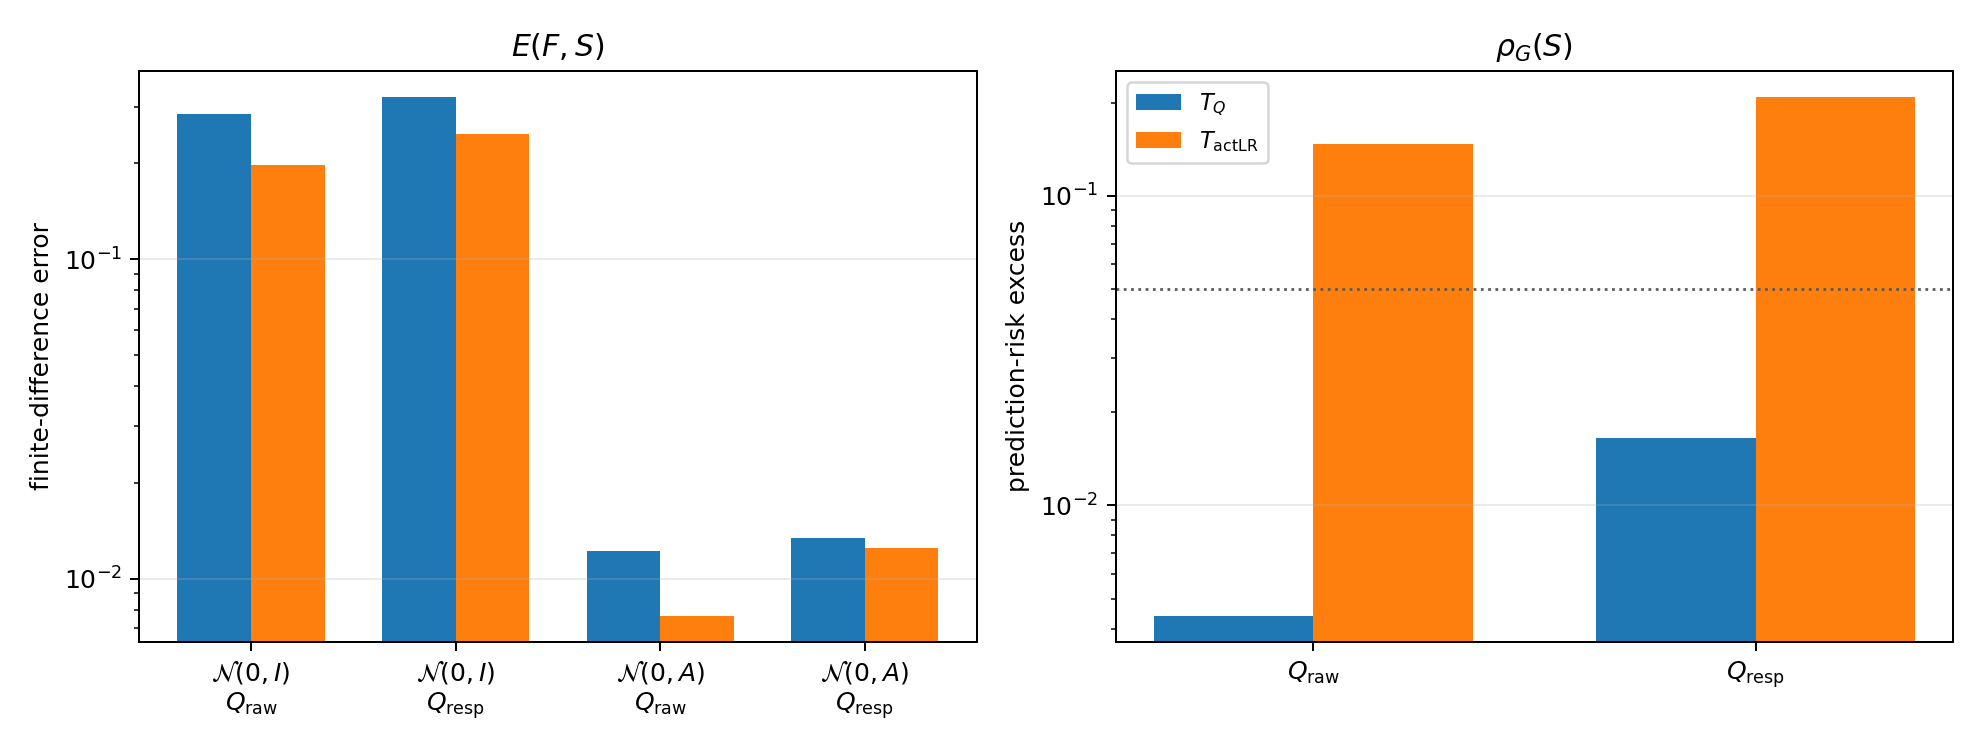
\includegraphics[width=0.90\linewidth]{../experiments/experiment_1_operator_certificate/results/actlr_comparison.png}
\caption{Experiment 1 same-span readout control. Left: finite-difference response error \(E(F,S)\)
on task and isotropic probes. Right: prediction-risk excess \(\rho_G(S)\), shown once per basis
because it is defined by the task covariance \(A\) rather than by the held-out probe law; the dotted
line marks the five-percent tolerance.
\(T_Q\) and actLR use the same activation coordinates \(Q^\top u\). actLR fits the transformer's
finite-difference responses with a free least-squares readout; \(T_Q\) uses the KRR-constrained
readout \(K_tQ\).}
\label{fig:exp1-actlr-control}
\end{figure}

The task-local nature of the certificate is also visible continuously. For this visualization we make
the comparison deliberately probe-law matched. For each mixing value, we draw perturbations
\[
u_\lambda=\sqrt{1-\lambda}\,u_{\mathrm{task}}+\sqrt{\lambda}\,u_{\mathrm{iso}},
\qquad
\lambda\in[0,1],
\]
where \(u_{\mathrm{task}}\sim\mathcal{N}(0,A)\) and \(u_{\mathrm{iso}}\sim\mathcal{N}(0,I)\). Thus
\(\lambda=0\) is the task-label probe law used for the certificate, while \(\lambda=1\) is the
isotropic off-distribution probe law. We then build a fresh response basis \(Q_\lambda\) from the
same mixed hidden finite differences that are used for the plotted evaluation. This is not a held-out
certificate; it is a fair matched-probe stress test asking whether the model's local KRR behavior
persists as perturbations leave the task-distributed directions. Figure~\ref{fig:exp1-probe-interpolation}
shows the degradation directly in finite-difference response error.

\begin{figure}[htbp]
\centering
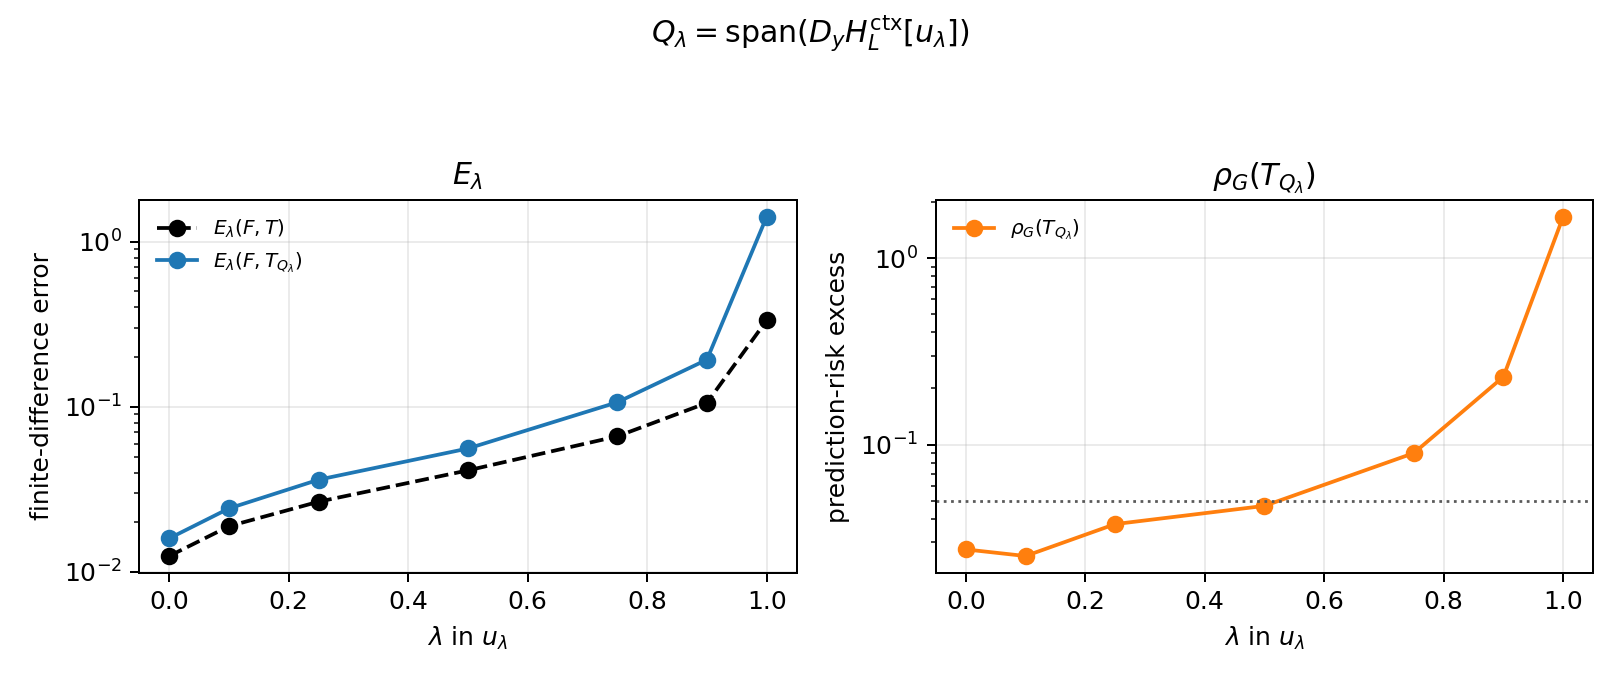
\includegraphics[width=0.70\linewidth]{../experiments/experiment_1_operator_certificate/results/probe_interpolation.png}
\caption{Experiment 1 task-to-isotropic probe interpolation with matched response bases. For each
\(\lambda\), \(Q_\lambda\) is built from the same mixed perturbations used in the plotted errors.
The transformer is locally KRR-like on task-distributed directions, but the finite-difference
operator error grows as the perturbations become isotropic.}
\label{fig:exp1-probe-interpolation}
\end{figure}

The finite-difference comparison is meaningful because the local response is close to additive:
at \(\varepsilon=10^{-3}\), the normalized additivity defect is \(3.69\times10^{-4}\) on task probes
and \(3.78\times10^{-3}\) on isotropic probes. Thus Experiment 1 establishes the basic endpoint
claim: on the task distribution, a compact activation subspace supports the KRR-constrained
operator that the transformer locally follows.

\FloatBarrier

\section{Experiment 2: Prediction-Risk Rank and Layerwise Availability}

Experiment 2 separates two facts that are easy to conflate. The prediction-risk rank \(r_T\) is an
intrinsic property of the finite KRR problem; it is computed from \(C_G=K_tA^{-1/2}\) before looking
at the transformer. The layerwise rank \(k_\ell^{5\%}\) is representation-dependent; it asks how
many directions from the transformer's layer-\(\ell\) response span are needed to reach
\(\rho_G\le0.05\). The diagnostic therefore asks not whether the hidden state has dimension
\(r_T\), but whether it contains an approximately \(r_T\)-dimensional KRR-sufficient subspace.

At each layer, we form the response span \(C_\ell\) from \(M_\ell=D_yH_\ell^{\mathrm{ctx}}\). The
span comes from activations, but the ordering inside it is KRR-targeted: we use the exact KRR
operator to find the best KRR-aligned prefixes available inside that span. Thus Experiment 2 measures
availability of a KRR-sufficient subspace, not whether the transformer autonomously selects this
basis. Prefixes \(Q_{\ell,k}\) are then evaluated by
\[
\rho_G(T_{Q_{\ell,k}})
=
\frac{\|(T-T_{Q_{\ell,k}})A^{1/2}\|_F^2}{R_{\mathrm{KRR}}+\eta_{\mathrm{num}}}.
\]
In Experiment 2 tables, ``cand. dim.'' is \(\dim C_\ell\) after numerical truncation, ``rank to
5\%'' is \(k_\ell^{5\%}\), ``best excess'' is \(\min_k\rho_G(T_{Q_{\ell,k}})\) over the tested
prefixes, and ``reach'' is the fraction of evaluated episodes for which some prefix reaches
\(\rho_G\le0.05\). A missing rank means the layer never reached the five-percent target in the
tested prefix range.

The small linear checkpoints calibrate the diagnostic in the regime where the answer is expected to
be simple. These trained models are
\path{linear_sweep_dx3.pt}, \path{linear_sweep_dx5.pt}, \path{linear_sweep_dx8.pt},
\path{linear_sweep_dx10.pt}, and \path{linear_sweep_dx15.pt}; all use the same 8-layer,
\(D=128\), 4-head architecture as Experiment 1, with the indicated input dimension \(d_x\). For
\(d_x=3,5,8,10,15\), with \(n_{\mathrm{ctx}}=47,n_{\mathrm{tgt}}=16\), the prediction-risk rank
matches the input dimension up to the target cap, and the final rank-to-five-percent matches
\(r_T\). This is not the main emergence result: in these linear tasks, the sufficient source
subspace is already visible very early. Its role is to show that the revised \(r_T\),
\(k_\ell^{5\%}\), and \(\rho_G\) diagnostic recovers the obvious low-dimensional answer.

\begin{table}[htbp]
\centering
\caption{Experiment 2 linear calibration. The table checks that the prediction-risk diagnostic
recovers \(r_T\approx d_x\) in simple linear tasks. ``First layer'' is the first layer whose response
span reaches \(\rho_G\le0.05\).}
\scriptsize
\setlength{\tabcolsep}{4pt}
\renewcommand{\arraystretch}{0.9}
\begin{tabular}{lrrrrr}
\toprule
Checkpoint & \(r_T\) & first layer & final cand. dim. & \(k_L^{5\%}\) & \(E_{\mathrm{task}}(F,T)\)\\
\midrule
\(d_x=3\)  & 3.0  & 0 & 27.5 & 3.0  & 0.00617\\
\(d_x=5\)  & 5.0  & 0 & 27.6 & 5.0  & 0.00918\\
\(d_x=8\)  & 8.0  & 0 & 40.1 & 8.0  & 0.01250\\
\(d_x=10\) & 10.0 & 0 & 40.4 & 10.0 & 0.01433\\
\(d_x=15\) & 14.9 & 2 & 46.6 & 14.9 & 0.01735\\
\bottomrule
\end{tabular}
\renewcommand{\arraystretch}{1}
\end{table}

The cleanest emergence result is instead the nonlinear checkpoint
\path{rbf_fixed_l3_nctx128_ntgt128_seed42.pt}, trained from scratch on the fixed RBF kernel with
lengthscale \(3.0\), \(d_x=5\), \(D=128\), 8 layers, 4 heads, \(n_{\mathrm{ctx}}=128\), and
\(n_{\mathrm{tgt}}=128\). We diagnose it in the same \(128\times128\) regime. The model itself is
locally close to exact KRR on task probes:
\[
E_{\mathrm{task}}(F,T)=0.0306.
\]
For this finite KRR problem, \(r_T\approx24.75\). Unlike the small linear sweep, the relevant
subspace is not already present at layer 0. It appears over the first few layers.

\begin{table}[htbp]
\centering
\caption{Experiment 2 main emergence result: selected layers of the RBF \(128\times128\) checkpoint.
Here \(r_T\approx24.75\). The response span is ordered by KRR usefulness before evaluating
\(\rho_G\).}
\scriptsize
\setlength{\tabcolsep}{4pt}
\renewcommand{\arraystretch}{0.9}
\begin{tabular}{rrrr}
\toprule
Layer & cand. dim. & rank to 5\% & \(\rho_G(T_{Q_{\ell,r_T}})\)\\
\midrule
0 & 16  & --   & 1.147\\
1 & 51  & 38.0 & 0.100\\
2 & 84  & 26.9 & 0.058\\
4 & 107 & 25.2 & 0.050\\
8 & 119 & 24.9 & 0.048\\
\bottomrule
\end{tabular}
\renewcommand{\arraystretch}{1}
\end{table}

The transition is the main point. Layer 0 has only a 16-dimensional response span and is far from
sufficient. By layer 2, a nearly task-rank subspace is visible; by layers 4 and 8,
\(k_\ell^{5\%}\) matches \(r_T\) to within finite-sample noise. The final response span is much
larger than \(r_T\), but it contains an approximately \(25\)-dimensional KRR-sufficient subspace.
Experiment 2 is therefore an availability diagnostic: it locates when the prediction-risk-rank
subspace becomes linearly available, before the label-space tests ask whether that subspace is
enough on ordinary model inputs.

\begin{figure}[htbp]
\centering
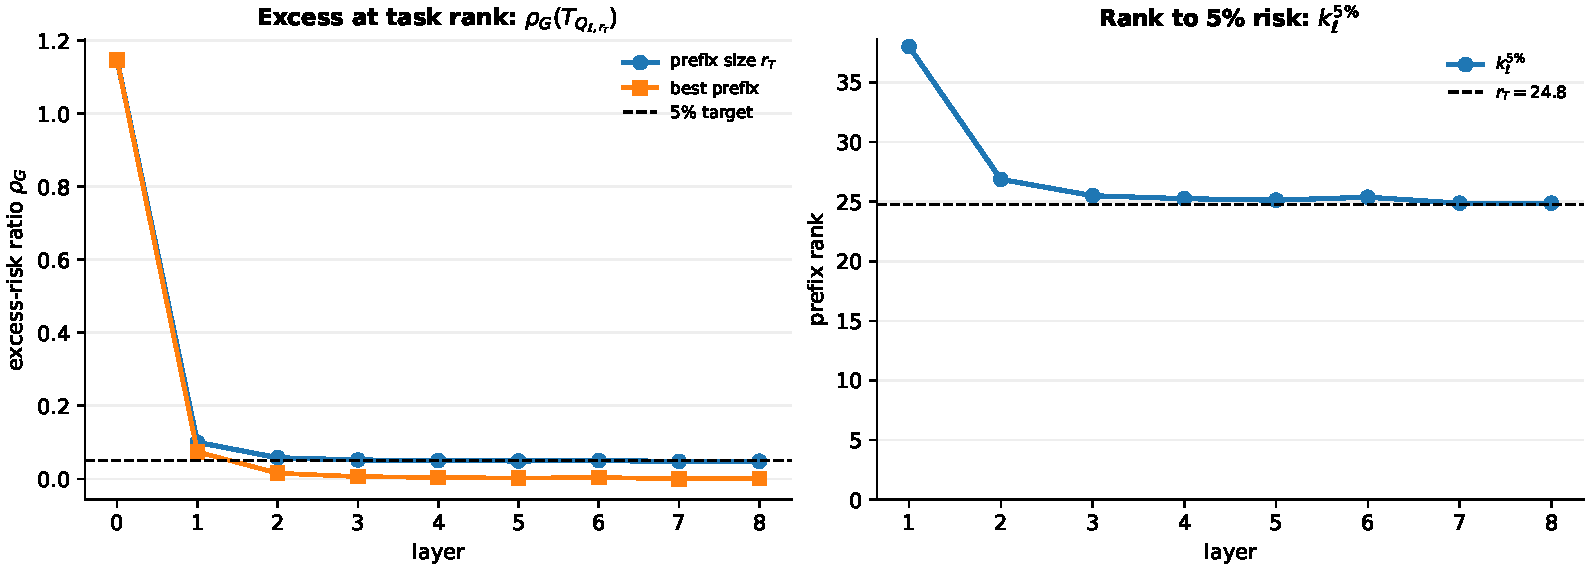
\includegraphics[width=0.95\linewidth]{../experiments/experiment_2_rank_emergence/results/rbf_128x128_seed42/emergence_response.pdf}
\caption{Experiment 2 layerwise emergence in the matched RBF \(128\times128\) checkpoint. The
candidate span is the response span \(C_\ell=\spanop(D_yH_\ell^{\mathrm{ctx}})\). Left:
the excess-risk ratio \(\rho_G\) for the prefix of size \(r_T\) and for the best prefix inside
\(C_\ell\); the dashed line is the five-percent target. Right: the first prefix rank
\(k_\ell^{5\%}\) that reaches the target, with the intrinsic prediction-risk rank \(r_T\) shown as a
dashed line. The disappearance of the large rank gap by the middle layers is the emergence signal.}
\label{fig:exp2-rbf-emergence}
\end{figure}

\subsection{Stress Cases: Response Availability Tracks Failure}

The \(d_x=40\) checkpoint \path{dx40_tau16_s122.pt} gives the cleanest warning against
over-reading availability. It is a scale-aware 8-layer, \(D=128\), 4-head linear-regression
checkpoint trained in a target-poor regime:
\[
n_{\mathrm{tgt}}=8,
\qquad
\tau(\Sigma)=\sum_{i=1}^{40}\frac{\lambda_i}{\lambda_i+\sigma^2}\le16,
\]
with \(n_{\mathrm{ctx}}\) sampled as a multiple of the effective dimension. The diagnostic instead
uses
\[
n_{\mathrm{ctx}}=47,\qquad n_{\mathrm{tgt}}=40,
\]
so it asks for a richer simultaneous target operator than the checkpoint saw directly in one
training episode. The checkpoint README reports
\[
\mathrm{MSE}/\mathrm{MSE}_{\mathrm{KRR}}=1.638,
\]
so this checkpoint is not an exact-KRR solver. Since the layerwise diagnostic is meant to track the
operator the transformer locally implements, the primary candidate span here is the response span
\(C_\ell=\spanop(D_yH_\ell^{\mathrm{ctx}})\): these are precisely the residual-stream directions
activated to first order by context-label perturbations.

\begin{table}[htbp]
\centering
\caption{\(d_x=40\) response-span stress test. Here \(r_T=21.0\) and
\(E_{\mathrm{task}}(F,T)=0.0939\). ``Reach'' is the fraction of episodes whose response span contains some prefix
with \(\rho_G\le0.05\).}
\scriptsize
\setlength{\tabcolsep}{4pt}
\renewcommand{\arraystretch}{0.9}
\begin{tabular}{rrrrr}
\toprule
Layer & cand. dim. & reach & \(\rho_G(T_{Q_{\ell,r_T}})\) & best \(\rho_G\)\\
\midrule
0 & 16.0 & 0.00 & 0.965 & 0.965\\
2 & 35.0 & 0.50 & 0.164 & 0.137\\
5 & 38.0 & 0.50 & 0.105 & 0.073\\
8 & 40.0 & 0.50 & 0.118 & 0.086\\
\bottomrule
\end{tabular}
\renewcommand{\arraystretch}{1}
\end{table}

The response span improves substantially over the first layers but does not become a reliable
five-percent KRR response. At the final layer, using the task-rank prefix gives
\(\rho_G(T_{Q_{L,r_T}})\approx0.118\); even the best response-span prefix remains at
\(\rho_G\approx0.086\), and only half the episodes reach the five-percent threshold at all. This is
the mechanistic counterpart of the checkpoint's non-optimal prediction ratio: the model has learned
a useful but imperfect target-rich KRR response.

Auxiliary raw-residual and union-span checks can find more KRR-aligned directions in this checkpoint,
but we do not treat those as evidence for the implemented operator. They are containment checks:
they show that some relevant information exists somewhere in the residual stream. The response span
is the stricter diagnostic for what the model actually uses in the local label-to-output map.

\begin{figure}[htbp]
\centering
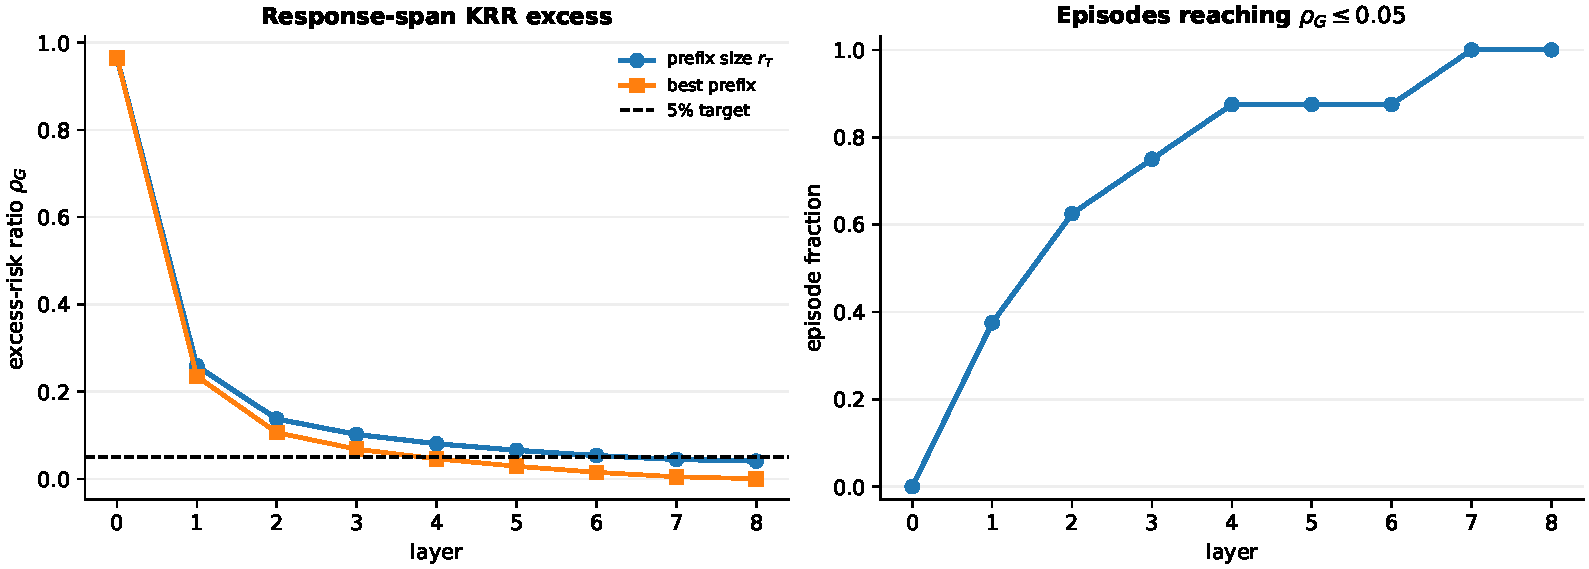
\includegraphics[width=0.95\linewidth]{../experiments/experiment_2_rank_emergence/results/dx40_target_rich/emergence_response_reach.pdf}
\caption{Experiment 2 \(d_x=40\) response-span stress case. Left: response-span excess risk at the
prediction-risk rank \(r_T\), together with the best prefix inside the response span. Both remain
above the five-percent target. Right: fraction of episodes in which any response-span prefix reaches
\(\rho_G\le0.05\). The response geometry improves but never becomes a reliable
prediction-risk-sufficient representation in the target-rich diagnostic regime.}
\label{fig:exp2-dx40-stress}
\end{figure}

We also reran the revised layerwise diagnostic on the older fixed-\(\ell=3\) RBF checkpoint
\path{rbf_fixed_l3_original.pt}, copied from \path{checkpoints/model_rbf_fixed_l3.pt}, at
\(n_{\mathrm{ctx}}=47\) and \(n_{\mathrm{tgt}}=16,64,128\). The final response-span summary is:

\begin{table}[htbp]
\centering
\caption{Older fixed-\(\ell=3\) RBF checkpoint, final-layer response diagnostic. The response span
continues to contain a near-sufficient KRR subspace as \(n_{\mathrm{tgt}}\) grows, but the realized
finite-difference operator becomes less clean.}
\label{tab:exp2-old-rbf}
\begin{tabular}{ccccc}
\toprule
\(n_{\mathrm{tgt}}\) & \(r_T\) & \(k_L^{5\%}\) & \(\rho_G(T_{Q_{L,r_T}})\) & \(E_{\mathrm{task}}(F,T)\)\\
\midrule
16  & 10.6 & 11.1 & 0.049 & 0.067\\
64  & 17.1 & 17.8 & 0.053 & 0.074\\
128 & 18.3 & 19.3 & 0.057 & 0.097\\
\bottomrule
\end{tabular}
\end{table}

Thus this older checkpoint shows a softer version of the same lesson: response availability can
improve with depth while the realized finite-difference operator remains less clean than in the
matched \(128\times128\) RBF regime.

\section{Experiment 3: On-Manifold Label-Space Use}

Experiments 1--2 show that a KRR-sufficient dual subspace is available. Experiment 3 asks whether
that subspace is enough when converted back into actual context labels, so the transformer is always
run on a valid input sequence.

Use \path{linear_baseline_dx5_L8.pt} on flat-spectrum linear episodes:
\[
d_x=5,\qquad n_{\mathrm{ctx}}=47,\qquad n_{\mathrm{tgt}}=16,\qquad \sigma^2=0.1.
\]
Run 32 episodes with seed \(31415\). For each episode, extract the raw final-state basis
\[
Q=[q_1,\ldots,q_k],
\qquad Q^\top A Q=I,
\]
with \(\tau_{\mathrm{sv}}=10^{-3}\) and \(r_{\max}=12\). The average extracted size is \(k=11.8\);
the intrinsic KRR risk rank is \(\mathbb{E}[r_T]=5\); and
\[
\mathbb{E}\,\rho_G(T_Q)=1.55\cdot10^{-3}.
\]

Define the label projections
\[
y_Q=AQQ^\top y,
\qquad
y_\perp=y-y_Q.
\]
Since
\[
Ty_Q=K_tA^{-1}AQQ^\top y=K_tQQ^\top y=T_Qy,
\]
feeding \(y_Q\) is the on-manifold version of evaluating the certified reduced KRR operator.

\begin{table}[htbp]
\centering
\caption{Experiment 3 label-space projection. Ratios are episode MSE divided by the original KRR
MSE. The KRR-input column reports the same label projection passed through KRR itself.}
\small
\setlength{\tabcolsep}{4pt}
\begin{tabular}{@{}lrrrr@{}}
\toprule
Input labels & mean MSE/KRR & median MSE/KRR & median KRR-input/KRR & median drift from \(F(y)\)\\
\midrule
\(y\) & 1.619 & 1.085 & 1.000 & 0\\
\(y_Q=AQQ^\top y\) & 1.602 & 1.090 & 0.9999 & \(2.91\cdot10^{-4}\)\\
\(y_\perp=y-y_Q\) & \(5.27\cdot10^3\) & \(1.77\cdot10^3\) & \(1.77\cdot10^3\) & 1.000\\
\bottomrule
\end{tabular}
\end{table}

The projected label stream \(y_Q\) preserves the model prediction and the KRR oracle. The
complement \(y_\perp\) is not useful: KRR itself fails on it by the same scale as the model.

\begin{figure}[htbp]
\centering
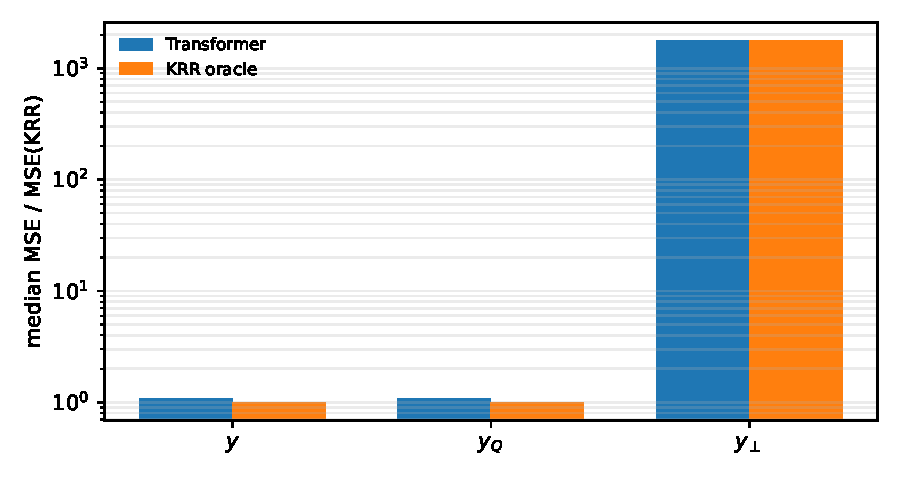
\includegraphics[width=0.72\linewidth]{../experiments/experiment_3_causal_surgery/results_label_space/label_space_mse_ratios.pdf}
\caption{Experiment 3 on-manifold label-space projection. The transformer and KRR oracle both
remain near the original KRR error on \(y_Q\), while both fail on \(y_\perp\).}
\label{fig:exp3-label-space-main}
\end{figure}

\FloatBarrier

\section{Experiment 4: Repair by Label-Space Projection}

Use the \(d_x=40\) checkpoint \path{dx40_tau16_s122.pt} in the target-rich diagnostic setting
\[
n_{\mathrm{ctx}}=47,\qquad n_{\mathrm{tgt}}=40,\qquad \log_{10}\lambda_1\in[-2,1].
\]
For each episode, form the final-layer response span, order it by KRR-targeted energy, and choose
the first prefix \(Q=Q_{8,k}\) satisfying \(\rho_G(T_{Q_{8,k}})\le0.05\), if such a prefix exists.

On a 200-episode bank with seed \(20260506\),
\[
\begin{array}{c|cccc}
\text{quantity} & \text{mean} & \text{median} & q_{25}\text{--}q_{75} & \text{tail / range}\\
\hline
\mathrm{MSE}_{\mathrm{model}}/\mathrm{MSE}_{\mathrm{KRR}}
& 84.96 & 1.14 & 1.03\text{--}1.37 & q_{90}=1.67,\ q_{99}=4.19,\ \max=1.67\cdot10^4\\
r_T & 23.29 & 25 & 19.75\text{--}28 & 1\text{--}32\\
k & 23.80 & 25 & 20\text{--}29 & 1\text{--}41\\
\rho_G(T_Q) & 0.0444 & 0.0441 & 0.0403\text{--}0.0471 & \Pr(\rho_G(T_Q)\le0.05)=194/200
\end{array}
\]
The bank is usually non-pathological and basis-present. Two episodes have base
\(\mathrm{MSE}/\mathrm{MSE}_{\mathrm{KRR}}\ge5\). On those two, run the transformer normally on
\[
y,\qquad y_Q=AQQ^\top y,\qquad y_\perp=y-y_Q.
\]

\begin{table}[htbp]
\centering
\caption{Experiment 4 target-rich label-space repair on the two bad episodes. All entries are
MSE/KRR ratios.}
\small
\setlength{\tabcolsep}{4pt}
\begin{tabular}{@{}lccc@{}}
\toprule
Input labels & mean & median & Reading\\
\midrule
\(y\) & \(8.37\cdot10^3\) & \(8.37\cdot10^3\) & pathological output\\
\(y_Q=AQQ^\top y\) & 1.079 & 1.079 & near-KRR repair\\
\(y_\perp=y-y_Q\) & \(6.00\cdot10^3\) & \(6.00\cdot10^3\) & complementary labels fail\\
\bottomrule
\end{tabular}
\end{table}

\[
\begin{array}{c|cccccc}
\text{bank id} & r_T & k & \rho_G(T_Q) &
\text{base} & y_Q & y_\perp\\
\hline
35 & 2 & 3 & 0.0482 & 1.67\cdot10^4 & 1.169 & 1.20\cdot10^4\\
184 & 1 & 1 & 0.0371 & 6.833 & 0.989 & 7.393
\end{array}
\]

Both outliers have \(\rho_G(T_Q)\le0.05\), so the KRR-sufficient response basis is present before
conditioning on bad outputs. Projecting the labels onto that basis brings the model back to
KRR-level error; the complementary labels do not.

\begin{figure}[htbp]
\centering
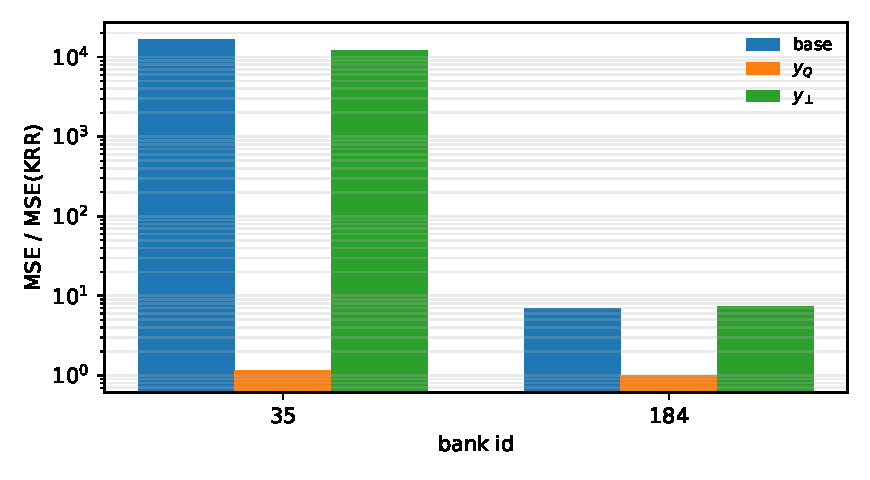
\includegraphics[width=0.72\linewidth]{../experiments/experiment_4_q_repair/results_label_space_target_rich/label_space_outliers.pdf}
\caption{Experiment 4 target-rich outliers. Feeding \(y_Q=AQQ^\top y\) repairs the two bad episodes;
feeding \(y_\perp=y-y_Q\) does not.}
\label{fig:exp4-label-repair-main}
\end{figure}

\FloatBarrier

\section{What Is Justified}

The experiments justify a bounded mechanistic claim:

\begin{quote}
For the tested checkpoint, geometries, perturbation scale, and task-label probe distribution, the
transformer's local label response is well approximated by a reduced KRR operator induced by a
compact context-side activation subspace. In successful settings, layerwise response spans contain
a prediction-risk-rank subspace whose induced reduced operator is prediction-risk sufficient, and
the corresponding label projection preserves the useful prediction signal.
\end{quote}

They do not justify stronger claims. They do not show that the transformer globally equals ridge
regression. They do not show that derivative matching at one sampled label vector implies equality
on a neighborhood. They do not show that the transformer literally executes the explicit algorithm
\[
y\mapsto QQ^\top y\mapsto K_tQQ^\top y
\]
as its internal program. They also do not show that architecture alone guarantees the behavior.
The prediction-risk rank calculation supplies a requirement for context-side subspaces; it is not
an SGD theorem.

The clean final formulation is:

\begin{quote}
The trained transformer locally realizes the ridge-regression label-response operator on
task-distributed directions. In the tested regime, this behavior is explained by a compact
context-side activation subspace whose induced reduced ridge operator is prediction-risk sufficient
at approximately the prediction-risk rank. The layerwise diagnostic tracks when such a subspace
becomes available; the label-space projection then asks whether the model can use the selected
subspace on ordinary input labels.
\end{quote}

\section{Logical Chain}

The argument can be read as a sequence of commitments, each narrower than the previous one:

\begin{enumerate}[label=\arabic*.]
\item Freeze the episode geometry \(G=(X_{\mathrm{ctx}},X_{\mathrm{tgt}})\).
\item Under fixed \(G\), ridge regression becomes \(T=K_tA^{-1}\).
\item Treat the transformer as a label map \(F:\R^{n_{\mathrm{ctx}}}\to\R^{n_{\mathrm{tgt}}}\).
\item Estimate the local response \(D_\varepsilon F(y)[u]\).
\item Test behavior by checking \(E_\varepsilon(F,T)\) on task-label probes.
\item Compute the prediction-risk rank \(r_T\) from \(C_G=K_tA^{-1/2}\) and \(R_{\mathrm{KRR}}\).
\item Extract activation-derived context-side candidate spans \(C_\ell\).
\item Order each candidate span by KRR-targeted energy and form prefixes \(Q_{\ell,k}\).
\item Construct the KRR-constrained reduced operator \(T_Q=K_tQQ^\top\).
\item Test subspace sufficiency with \(\rho_G(T_Q)\).
\item Test model-subspace alignment with \(E_\varepsilon(F,T_Q)\).
\item Convert certified \(Q\) into label projections \(y_Q=AQQ^\top y\) and \(y_\perp=y-y_Q\).
\item Run the model normally on \(y_Q\) and \(y_\perp\) to test on-manifold use and repair.
\end{enumerate}

This is the full mechanism story: behavioral similarity, a KRR-structured activation certificate,
prediction-risk-rank sufficiency, layerwise emergence of the relevant subspace, and on-manifold
label-space use.

\end{document}
